\documentclass{beamer}
\usepackage{microtype}
\usepackage{default}

\usetheme{simple}
\usepackage{fontspec}
\usepackage{graphicx}
\usepackage[utf8]{inputenc}
\setmainfont{Fira Sans}

\newfontfamily\DejaSans{DejaVu Sans}
\setbeamerfont{title}{family=\texttt,size=\huge}
\usepackage[scale=2]{ccicons}
\title{The i-score interactive sequencer}
\subtitle{an intermedia sequencer for interactive scenarios authoring}
\date{\today}
\author{Jean-Michaël Celerier, Théo de la Hogue}
\institute{LaBRI, Blue Yeti, GMEA }
\date{January 30, 2016}
\begin{document}
    
\maketitle

\begin{frame}
    \frametitle{The problem}        
\end{frame}

\begin{frame}
    \frametitle{Example installations}        

    \begin{figure}
        \centering
        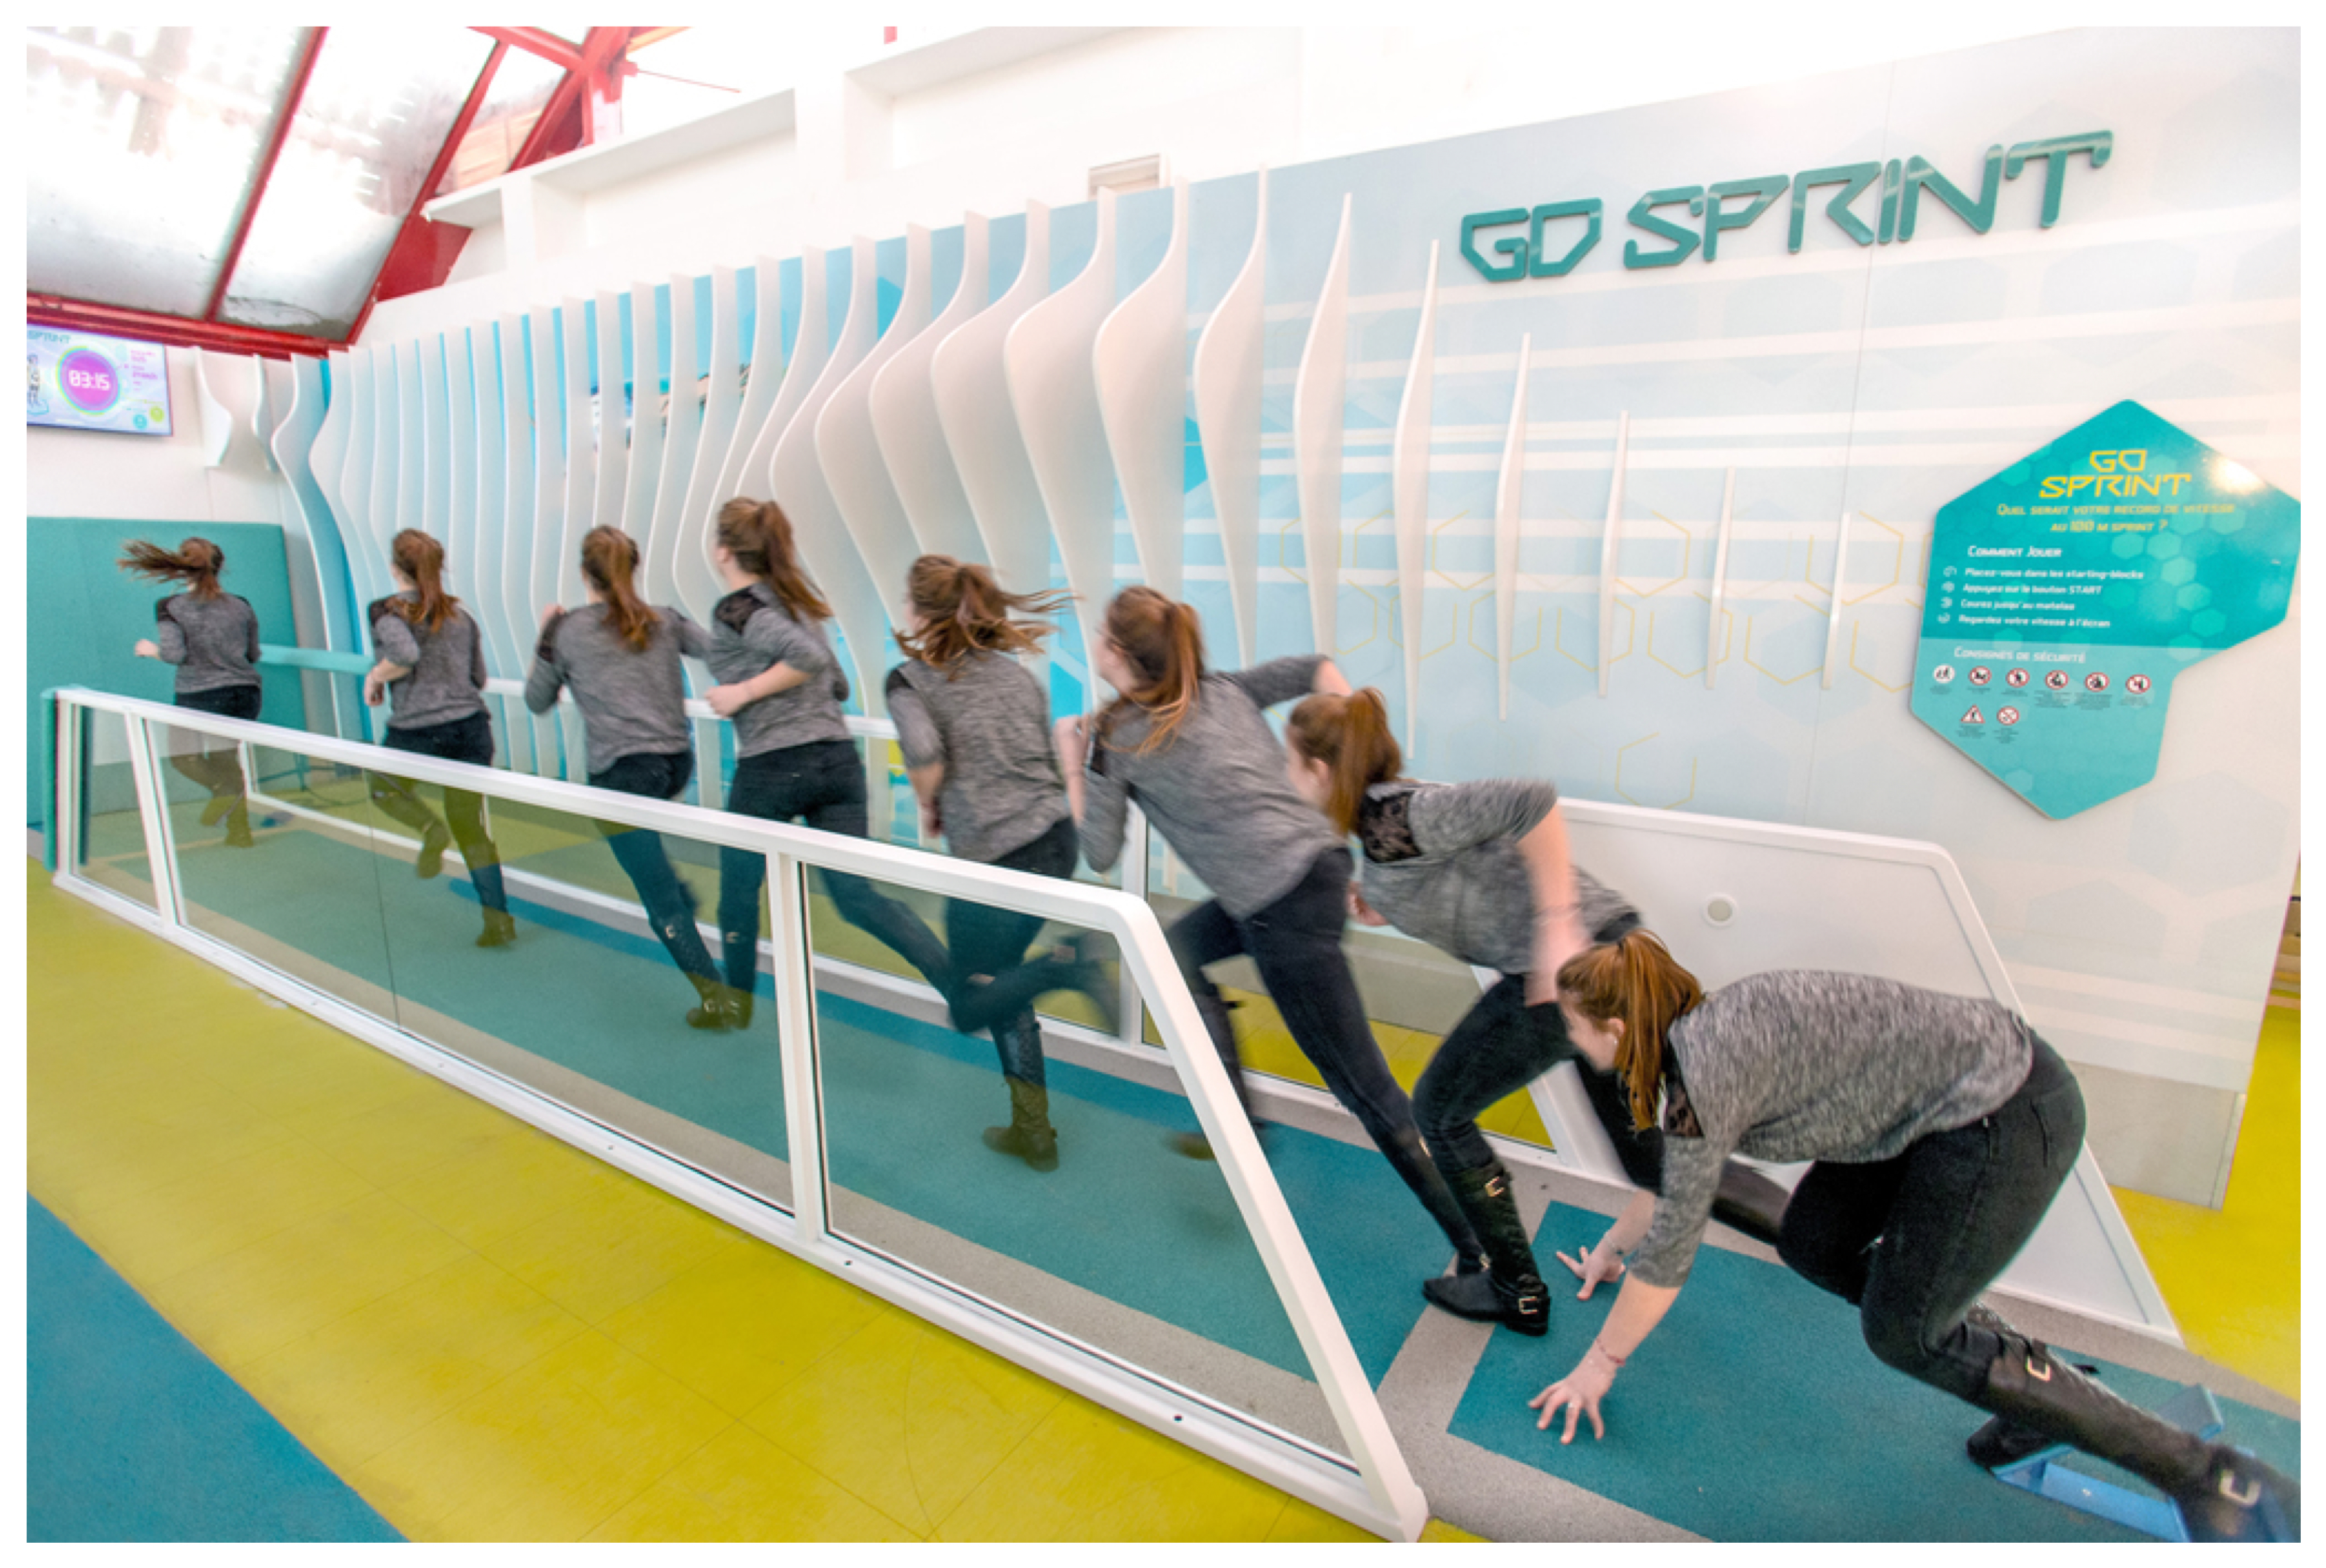
\includegraphics[width=0.9\textwidth]{images/futuroscope.jpg}
        \caption[]{Futuroscope, France. Blue Yeti}
    \end{figure}
\end{frame}


\begin{frame}
    \frametitle{Example installations}        
    robots
    ensatt
    pascal
    
\end{frame}

\begin{frame}
    \frametitle{Screenshot}        
\end{frame}


\begin{frame}
    \frametitle{Agencies involved}
    ANR
    
    LaBRI
    
    GMEA
    
    Blue Yeti
    
\end{frame}

    \begin{frame}
        \frametitle{What i-score is : }
        \begin{itemize}        
        \item Visual programming language for interactive multimedia applications        
        \item Free software : GPL v3 (UI) \& LGPL v2.1 (Engine)
        \item C++ (Qt, CMake)        
        \item Linux / OS X / Windows        
        \item Alpha-quality \DejaSans{☹}
        \end{itemize}
    \end{frame}
    \begin{frame}
        \frametitle{What i-score is not : }
        \begin{itemize}
            \item Audio sequencer        
            \item Video sequencer        
            \item PureData or Ableton Live       
            \item Bug-free
        \end{itemize}
    \end{frame}
    
    \begin{frame}
        \frametitle{Inter-operability}
        Max, PureData, Unity, OpenFrameworks, Processing, Jamoma, Modul8, Millumin, Quartz Composer, Qt...
    \end{frame}
    
    \begin{frame}
        \centering \Huge Demonstration
    \end{frame}
    
    \begin{frame}
        \frametitle{Automations, mappings}
        
    \end{frame}
    
    \begin{frame}
        \frametitle{Javascript}
        
    \end{frame}
    
    \begin{frame}
        \frametitle{Hierarchy}
        
    \end{frame}
    
    \begin{frame}
        \frametitle{Spatial automations}
        
    \end{frame}
    
    \begin{frame}
        \frametitle{Future : audio ?}
        
    \end{frame}

\begin{frame}
    \frametitle{Future : distribution ?}
    
\end{frame}

\begin{frame}
    \frametitle{Future : other features}
    
    \begin{itemize}
    \item MIDI, WebSockets support
    \item Some level of patching, like Pd
    \item Complete remote-control abilities; currently execution can be followed via a web page.
    \end{itemize}
\end{frame}

\begin{frame}
    \frametitle{Contributing}    
    \begin{itemize}
    \item UX, UI (mock-ups were done but not entirely implemented)
    \item Documentation, writing demo scenarios
    \item Translations    
    \item Implement the Minuit protocol in your software with the OSSIA API    
    \item Many "low-hanging fruit" TODOs
    \item Mobile devices ports : 
    \begin{itemize}
        \item Android : builds and run but requires adapted UI.
        \item Web port : with PNaCl, runs but crashes. Will open the way to WebAssembly. 
        \item iDevices (many artists use them).
    \end{itemize}
\end{itemize}
    
\end{frame}



\begin{frame}
    \frametitle{Links}
    \begin{itemize}
        \item \textbf{Grab a release !} :~\\ \url{github.com/OSSIA/i-score/releases}. 
        \item \textbf{Protocols and implementations} :~\\
        \url{github.com/OSSIA}
    \end{itemize}
        
    \centering
    \vspace{2cm}
    \Large{Thanks ! Questions ?}
    \vspace{2cm}
    
    \small{Credits: 'simple' Beamer theme, Facundo Muñoz; Fira font}
\end{frame}    
\end{document}
